\documentclass{article}
% translate with >> pdflatex -shell-escape <file>

% This file is an extract of the PGFPLOTS manual, copyright by Christian Feuersaenger.
% 
% Feel free to use it as long as you cite the pgfplots manual properly.
%
% See
%   http://pgfplots.sourceforge.net/pgfplots.pdf
% for the complete manual.
%
% Any required input files (for <plot table> or <plot file> or the table package) can be downloaded
% at
% http://www.ctan.org/tex-archive/graphics/pgf/contrib/pgfplots/doc/latex/
% and
% http://www.ctan.org/tex-archive/graphics/pgf/contrib/pgfplots/doc/latex/plotdata/

\usepackage{pgfplots}
\pgfplotsset{compat=newest}

\pagestyle{empty}
\usepackage{textcomp}

\begin{document}
% \usepackage{textcomp}
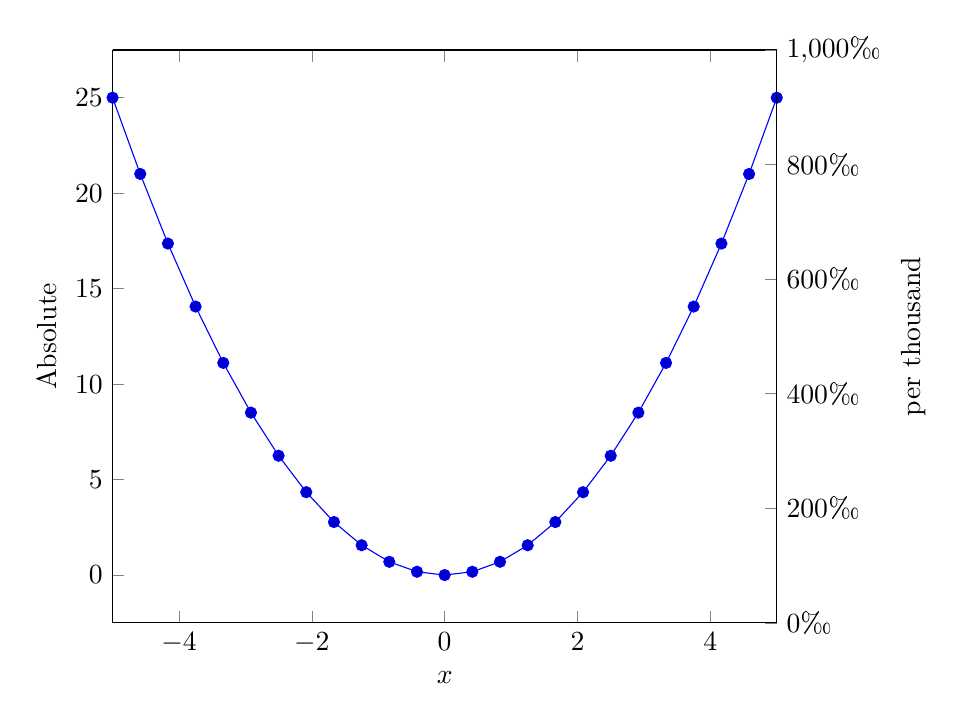
\begin{tikzpicture}
  \begin{axis}[
    scale only axis,
    xmin=-5,xmax=5,
    axis y line*=left,%'*' avoids arrow heads
    xlabel=$x$,
    ylabel=Absolute]
  \addplot {x^2};
  \end{axis}
  
  \begin{axis}[
    scale only axis,
    xmin=-5,xmax=5,
    ymin=0,ymax=1000,
    yticklabel=
{$\pgfmathprintnumber{\tick}$\textperthousand},
    axis y line*=right,
    axis x line=none,
    ylabel=per thousand]
  \end{axis}
\end{tikzpicture}
\end{document}
